% Name: Digital control loop
% Description: A computer closes the loop around a continuous plant through an analog-to-digital converter and a zero-order hold.
% Tags: digital control, sampling, zero-order hold, control systems

\usetikzlibrary{arrows.meta, positioning, fit}

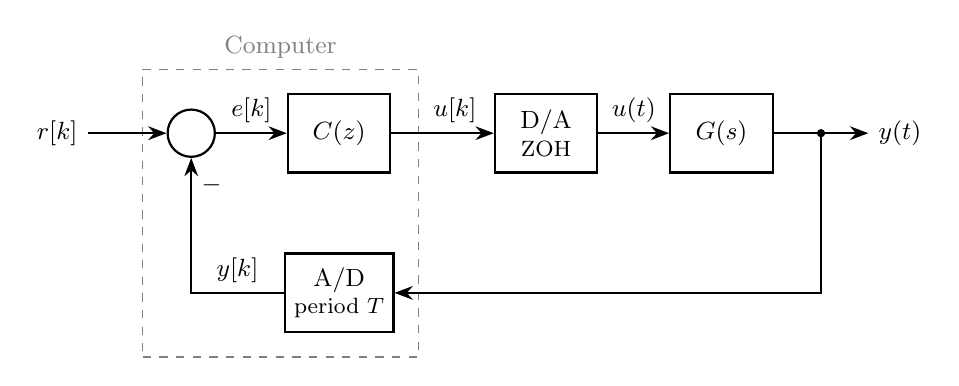
\begin{tikzpicture}[
  node distance=6mm and 9mm,
  every node/.style={font=\small},
  block/.style={draw, thick, minimum height=10mm, minimum width=13mm, align=center},
  sum/.style={draw, thick, circle, inner sep=0pt, minimum size=6mm},
  group/.style={draw, dashed, gray, inner sep=3mm},
  arrow/.style={-{Stealth}, thick},
]
  \node[sum] (sum) {};
  \node[block, right=of sum] (ctrl) {$C(z)$};
  \node[block, right=13mm of ctrl] (dac) {D/A\\[-1pt] \footnotesize ZOH};
  \node[block, right=of dac] (plant) {$G(s)$};
  \node[block, below=10mm of ctrl] (adc) {A/D\\[-1pt] \footnotesize period $T$};
  \node[group, fit=(sum)(ctrl)(adc), label={[gray]above:Computer}] {};

  \draw[arrow] ([xshift=-10mm]sum.west) node[left] {$r[k]$} -- (sum);
  \draw[arrow] (sum) -- node[above] {$e[k]$} (ctrl);
  \draw[arrow] (ctrl) -- node[above, pos=0.62] {$u[k]$} (dac);
  \draw[arrow] (dac) -- node[above] {$u(t)$} (plant);
  \draw[arrow] (plant.east) -- ++(12mm,0) coordinate (out) node[right] {$y(t)$};
  \draw[arrow] ([xshift=-6mm]out) |- (adc);
  \draw[arrow] (adc) -| node[pos=0.25, above] {$y[k]$} node[pos=0.9, right] {$-$} (sum);
  \fill ([xshift=-6mm]out) circle (1.5pt);
\end{tikzpicture}
